\chapter{量子统计}
\section{粒子的量子描述}
\section{玻色分布和费米分布}
对于玻色系统
\begin{equation}
    \Omega=\prod_l\frac{(\omega_l+a_l-1)}{a_l!(\omega-1)!}
\end{equation}
对应的最概然分布为:
\begin{equation}
    a_l=\frac{\omega_l}{e^{\alpha+\beta\varepsilon_l}-1}.
\end{equation}
称为玻色爱因斯坦分布。


对于费米系统 
\begin{equation}
    \prod_l\frac{\omega_l!}{a_l!(\omega_l-a_l)!}
\end{equation}
对应的最概然分布为
\begin{equation}
    a_l=\frac{\omega_l}{e^{\alpha+\beta\varepsilon_l}+1}.
\end{equation}
称为费米狄拉克分布。

当$a_l\ll \omega_l$时,二者都等价于玻尔兹曼分布,即经典情形。

\section{玻色系统和费米系统中热力学量的表达式}
\subsection{玻色系统}
对于玻色系统,引入巨配分函数:
\begin{equation}
    \Xi=\prod_l\Xi_l=\prod_l\left(1-e^{-\alpha-\beta\varepsilon_l}\right)^{-\omega_l}.
\end{equation}
取对数为:
\begin{equation}
    \ln\Xi=-\sum_l\omega_l\ln(1-e^{-\alpha-\beta\varepsilon_l}).
\end{equation}
系统总粒子数为
\begin{equation}
    N=-\pp{}{\alpha}\ln\Xi.
\end{equation}
系统内能为:
\begin{equation}
    U=-\pp{}{\beta}\ln \Xi.
\end{equation}
压强为:
\begin{equation}
    p=\frac{1}{\beta}\pp{}{V}\ln\Xi.
\end{equation}
由于
\begin{equation}
    \d S=\frac{1}{T}\left(\d U-p\d V -\mu\d\bar{N}\right).
\end{equation}
可以得到
\begin{equation}
    \beta=\frac{1}{kT}, \alpha =-\frac{\mu}{kT}.
\end{equation}
积分可以得到:
\begin{equation}
    S=k\ln\Omega
\end{equation}
即玻尔兹曼关系。

\subsection{费米系统}
费米系统的巨配分函数为:
\begin{equation}
    \Xi=\prod_l\left(1+e^{-\alpha-\beta\varepsilon_l}\right)^{\omega_l}.
\end{equation}
其余与玻色系统类似。

\section{量子系统的去经典化}
在体积$V$内,能量范围$[\varepsilon,\varepsilon+\d \varepsilon]$内,分子可能为微观状态数目为:
\begin{equation}
D(\varepsilon)\d \varepsilon=g \frac{V}{4\pi^2\hbar^3\varepsilon}\left(2m\varepsilon\right)^{3/2}\d\varepsilon.    
\end{equation}
其中$g$为可能存在自旋而引入的简并度。

系统的总粒子数和内能可以表示为:
\begin{equation}
    N=\int \d\varepsilon D(\varepsilon) \frac{1}{e^{\alpha+\beta\varepsilon}\pm1}=g \frac{V}{4\pi^2\hbar^3}\left(2m\right)^{3/2}\int\frac{\varepsilon^{1/2}}{e^{\alpha+\beta\varepsilon}\pm1} \d\varepsilon
\end{equation}
\begin{equation}
    U=\int \varepsilon\d\varepsilon D(\varepsilon) \frac{1}{e^{\alpha+\beta\varepsilon}\pm1}=g \frac{V}{4\pi^2\hbar^3}\left(2m\right)^{3/2}\int \frac{\varepsilon^{3/2}}{e^{\alpha+\beta\varepsilon}\pm1} \d\varepsilon
\end{equation}

换元$x=\equiv \beta\varepsilon$,则有 
\begin{align}
    N&=g \frac{V}{4\pi^2\hbar^3}\left(2mkT\right)^{3/2}\int\frac{x^{1/2}}{e^{\alpha+x}\pm1} \d x\\
    U&=g \frac{V}{4\pi^2\hbar^3}\left(2mkT\right)^{3/2}kT\int\frac{x^{3/2}}{e^{\alpha+x}\pm1} \d x.
\end{align}

这里为了方便,我们将费米系统放在$\pm/\mp$符号的上方,玻色系统在下方。

在$e^{\alpha}$比较大的情形,有以下近似:
\begin{equation}
    \frac{1}{e^{\alpha+x}\pm1}=e^{-\alpha-x}(1\mp e^{-\alpha-x}).
\end{equation}
只保留其中第一项就是经典近似,这里在弱简并的情形下,我们保留其中前两项。

代入积分可以得到
\begin{align}
    N&=g\left(\frac{mkT}{2\pi\hbar^2}\right)^{3/2}Ve^{-\alpha}\left(1\mp\frac{1}{2\sqrt{2}e\alpha}\right)\\
    U&=\frac{3}{2}\left(\frac{mkT}{2\pi\hbar^2}\right)^{3/2}VkTe^{-\alpha}\left(1\mp\frac{1}{4\sqrt{2}e\alpha}\right)
\end{align}
二者相除,只保留一阶小量,可以得到
\begin{equation}
    U=\frac{3}{2}NkT\left(1\pm\frac{e^{-\alpha}}{4\sqrt{2}}\right).
\end{equation}
同样仅保留一阶小量 
\begin{equation}
    e^{-\alpha}=\frac{N}{V}\left(\frac{2\pi\hbar^2}{mkT}\right)^2\frac{1}{g} \to \frac{1}{g}N\lambda^3.
\end{equation}
那么
\begin{equation}
    U=\frac{3}{2}NkT\left(1\pm\frac{1}{4\sqrt{2}g}n\lambda^3\right).
\end{equation}
显然,当简并度较大时,该式可以近似为经典情形。
\section{Bose-Einstein condensation}
考虑一个自旋为0的全同玻色子系统,其化学能为:
\begin{equation}
    \mu=-\frac{\alpha}{kT}.
\end{equation}
根据玻色分布处于能级$\varepsilon_l$的粒子数为:
\begin{equation}
    a_l=\frac{\omega_l}{e^{\frac{\varepsilon_l-\mu}{kT}}-1}
\end{equation}
粒子数不可能为负,这要求体系的最低能级$\varepsilon_0>\mu$.

化学势会随着临界温度的升高而降低,达到临界温度$T_c$时,化学势达到条件$\mu\to 0$ ,此时:
\begin{equation}
    2\pi\left(\frac{2mkT_c}{4\pi^2\hbar^2}\right)^{3/2}\int_0^{+\infty}\frac{x^{1/2}}{e^x-1}\d x=n, \ x=\frac{\varepsilon}{kT_c}.
\end{equation}
积分可以得到临界温度为:
\begin{equation}
    T_c=\frac{1}{2.612^{3/2}}\frac{2\pi\hbar^2}{mk}n^{2/3}.
\end{equation}

当温度小于临界温度时, 粒子会大量聚集在基态,这种现象称为玻色爱因斯坦凝聚。
\begin{figure}[htb]
    \centering 
    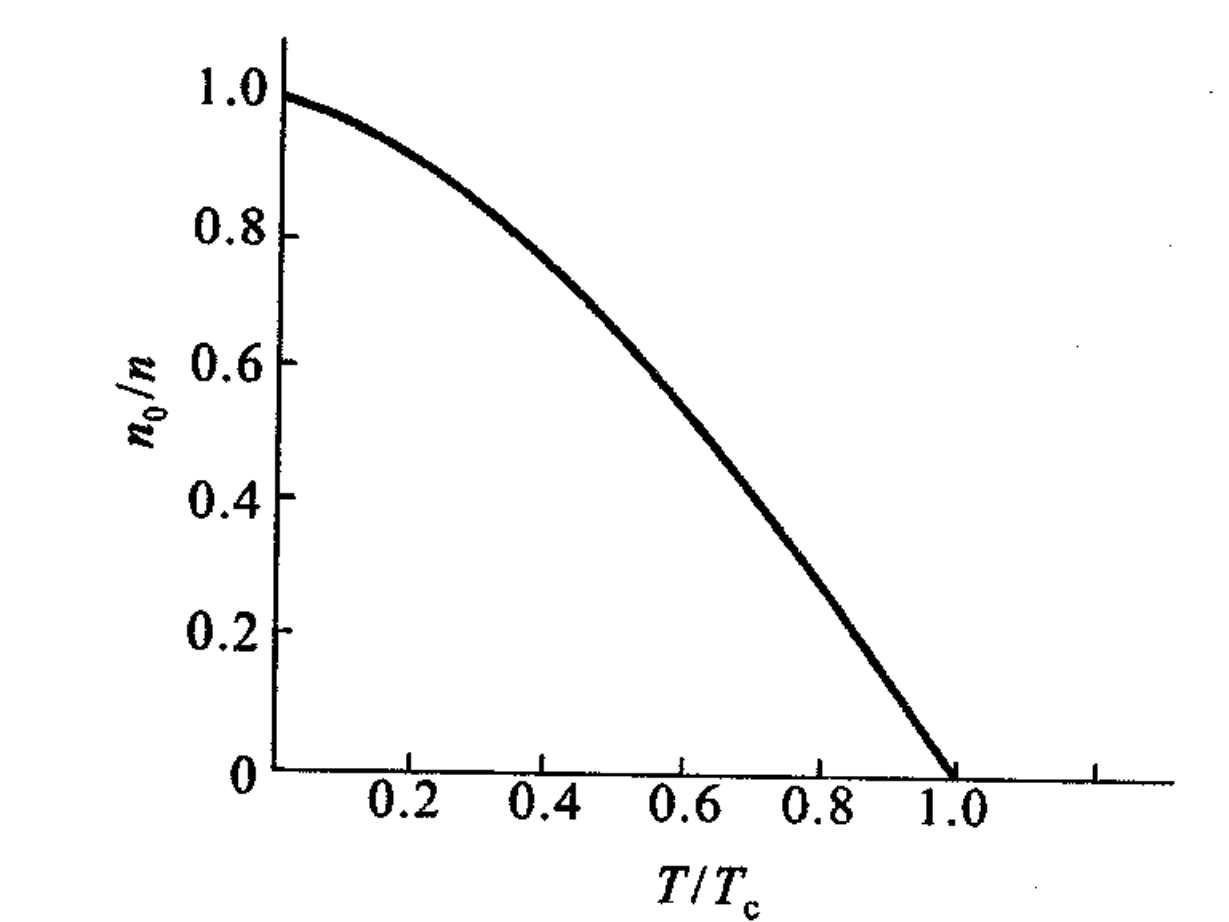
\includegraphics[width=0.5\linewidth]{fig/ch4_BEcom.png}
    \label{BEcom}
    \caption{玻色爱因斯坦凝聚现象。当温度小于临界温度时,玻色子会大量聚集于基态。\cite{wang_2003}}
\end{figure}
\section{Photon Gas}
\section{Free electrons in Metal}
\section{Quantum Hall Effect}
